
\documentclass[pdflatex,sn-basic,Numbered]{sn-jnl}

\usepackage{graphicx}%
\usepackage{multirow}%
\usepackage{amsmath,amssymb,amsfonts}%
\usepackage{xcolor}%
\usepackage{booktabs}%
\usepackage{url}%
\usepackage{float}%
\usepackage{tabularx}%
\newcolumntype{Y}{>{\centering\arraybackslash}X}%
\usepackage{array}%
\usepackage{colortbl}%
\usepackage{geometry}%

\definecolor{ourrow}{RGB}{242,247,252}

\geometry{top=3cm, bottom=3cm, footskip=1cm}

\graphicspath{{images/}}

\setcounter{topnumber}{4}
\setcounter{bottomnumber}{2}
\setcounter{totalnumber}{6}
\renewcommand{\topfraction}{0.95}
\renewcommand{\bottomfraction}{0.85}
\renewcommand{\textfraction}{0.05}
\renewcommand{\floatpagefraction}{0.80}
\setlength{\textfloatsep}{8pt plus 2pt minus 2pt}
\setlength{\floatsep}{8pt plus 2pt minus 2pt}
\setlength{\intextsep}{8pt plus 2pt minus 2pt}

\raggedbottom


\begin{document}

\title{A Reliability-Oriented and Interpretable Machine Learning Framework for Diabetes Analytics Using the CDC BRFSS Dataset}

% First Author - Equal Contribution
\author[1]{\fnm{Dat} \sur{Phan Tuan}}
\email{ptundatwork@gmail.com}

% Second Author
\author[1]{\fnm{Khang} \sur{Lam Huynh}}
\email{khanglhse200666@fpt.edu.vn}

% Third Author - Equal Contribution
\author[1]{\fnm{Linh} \sur{Nguyen Hoang}}
\email{linhnh67@fe.edu.vn}

% Affiliation
\affil*[1]{
    \orgdiv{Faculty of Information Technology},
    \orgname{FPT University},
    \orgaddress{
        \city{Ho Chi Minh City},
        \country{Vietnam}
    }
}


\abstract{
Machine-learning models based on self-reported health indicators may support diabetes screening, but class imbalance, threshold selection, and probability calibration complicate their evaluation. This study analyzed 253,680 records from the unweighted CDC BRFSS 2015 Diabetes Health Indicators dataset, with 13.93\% belonging to the positive class. Logistic Regression, Decision Tree, Random Forest, and XGBoost were compared using five-fold stratified cross-validation on an 80\% development set, with PR-AUC as the primary selection metric. XGBoost achieved the highest mean PR-AUC of 0.4359. A threshold of 0.13 was selected from development out-of-fold predictions under a prespecified Recall $\geq 0.80$ constraint. On the independent internal holdout set, XGBoost achieved PR-AUC of 0.4238 and ROC-AUC of 0.8272. At the selected threshold, Recall reached 80.99\%, Precision 29.91\%, and F1-score 0.4369. Calibration assessment yielded a Brier score of 0.0974, a slope of 0.9589, and an intercept of $-0.0515$. SHAP identified self-rated general health, high blood pressure, age, BMI, and high cholesterol as the most influential predictors. SHAP and multivariable likelihood-ratio rankings shared all ten highest-ranked features (Jaccard similarity = 1.0000; Spearman correlation = 0.9338), whereas seven features overlapped with univariate effect-size rankings (Jaccard similarity = 0.5385). These findings describe internal screening performance and agreement between feature-importance measures, without establishing clinical validity, causality, or population-level generalizability.
}


\keywords{Diabetes Risk Screening, BRFSS, Machine Learning, XGBoost, Calibration, SHAP, Statistical Association, Explainable Artificial Intelligence}

\maketitle


\section{Introduction}
\label{sec:intro}

Diabetes can lead to cardiovascular, kidney, nerve, and vision complications, making early identification of people at higher risk important for screening and preventive care~\citep{ullah2022detecting,olisah2022diabetes,zhang2024prediabetes}.
The Behavioral Risk Factor Surveillance System (BRFSS) collects self-reported demographic, behavioral, and health information without laboratory measurements. Previous research has used these indicators, including age, BMI, blood pressure, cholesterol, physical activity, and general health, to develop diabetes prediction models~\citep{xie2019diabetes,li2024gaxgboost,muhammad2025brfss}.

Only 13.93\% of records in the analyzed BRFSS 2015 dataset belong to the positive class. With such an imbalance, high Accuracy does not necessarily mean that a model detects positive cases well. We therefore used PR-AUC for model selection and Recall to guide the screening threshold~\citep{saito2015precisionrecall}. The threshold was chosen using development data before holdout evaluation, since changing it after examining test results could bias the reported performance. Calibration was assessed separately through the Brier score, calibration slope, and intercept. A model may distinguish between classes reasonably well while still producing probabilities that differ from observed outcome frequencies~\citep{huang2020calibration}.

SHAP helps explain how individual predictors contribute to model predictions, but it does not establish causal relationships~\citep{lundberg2017unified,lundberg2020trees}. To examine these explanations, we compared global SHAP importance with likelihood-ratio Chi-square contributions from multivariable Logistic Regression. Univariate effect sizes were used as a supplementary comparison. These measures do not always produce the same rankings because a predictor may be strongly associated with the outcome on its own but contribute less when other predictors are considered.

The analysis followed a development and evaluation pipeline using the original imbalanced CDC BRFSS 2015 Diabetes Health Indicators dataset. Logistic Regression, Decision Tree, Random Forest, and XGBoost were compared through five-fold stratified cross-validation, with mean PR-AUC determining model selection. A screening threshold was then selected from out-of-fold development predictions under a prespecified Recall constraint. Once the model and threshold were fixed, performance was measured on an independent internal holdout set using classification metrics, discrimination measures, bootstrap confidence intervals, and calibration. SHAP was applied to the final model, with its feature rankings compared against the statistical analyses.

The main contribution is not a new classifier or explanation method. Instead, the focus is on keeping model selection, threshold choice, and final evaluation separate while examining both predictive performance and feature importance. We consider this separation important because decisions made after seeing holdout results can make performance estimates less reliable. The findings are limited to the analyzed, unweighted BRFSS sample and do not establish clinical diagnoses, causal effects, or national population estimates. Data-processing scripts, SQL validation queries, statistical analyses, machine-learning code, figures, and reproducibility checks are available at \url{https://github.com/AI-Peak/Diabetes-Analytics}.



\section{Related Work}
\label{sec:related}

Diabetes prediction has been studied using both survey and clinical data. Xie et al.~\citep{xie2019diabetes} compared five classifiers on BRFSS 2014 and examined adjusted associations through multivariable regression. Li et al.~\citep{li2024gaxgboost} combined class balancing, GA-optimized XGBoost, stacking, and SHAP. Other BRFSS studies have also used tree-based models and SHAP~\citep{majcherek2025aidriven,muhammad2025brfss}. However, reviews report considerable differences in data preparation, validation, and reporting~\citep{mohsen2023scoping}. These differences make comparisons across studies difficult.

Class imbalance is one reason why evaluation methods matter. When positive cases are uncommon, Precision--Recall analysis provides information that ROC analysis alone may miss~\citep{saito2015precisionrecall}. Prediction-model guidelines recommend separating development decisions from final evaluation and examining more than discrimination scores~\citep{efthimiou2024developing,collins2024evaluation}. TRIPOD+AI and PROBAST+AI further address reporting quality, risk of bias, and applicability~\citep{collins2024tripodai,moons2025probastai}. Calibration also matters when predicted probabilities are interpreted as risk estimates~\citep{huang2020calibration}.

SHAP has been widely used to explain model predictions~\citep{lundberg2017unified,lundberg2020trees}, including in diabetes research~\citep{lugner2024predictors,prendin2023shap}. However, SHAP importance and statistical association measure different things. A predictor may show a strong association with diabetes on its own but contribute less to a model after other predictors are included. Neither measure establishes causality.

Given the existing work on XGBoost and SHAP, we focus on how model performance and explanations are evaluated. The analysis combines cross-validated model selection, threshold selection from development predictions, independent internal holdout evaluation, bootstrap confidence intervals, and calibration. SHAP rankings are then compared with multivariable likelihood-ratio contributions and univariate effect sizes. The aim is to examine whether these methods identify similar predictors, without treating their agreement as evidence of clinical validity.




\section{Materials and Methods}
\label{sec:materialsandmethods}

Figure~\ref{fig:methodology_pipeline} summarizes the analysis pipeline.
The workflow comprised data validation, statistical association analysis,
model development and selection, threshold selection, holdout evaluation,
calibration assessment, and SHAP-based explanation.
The complete workflow can be executed end to end through the
repository-level pipeline script, and the figures and tables reported below
are regenerated by the same code.

\begin{figure}[H]
\centering
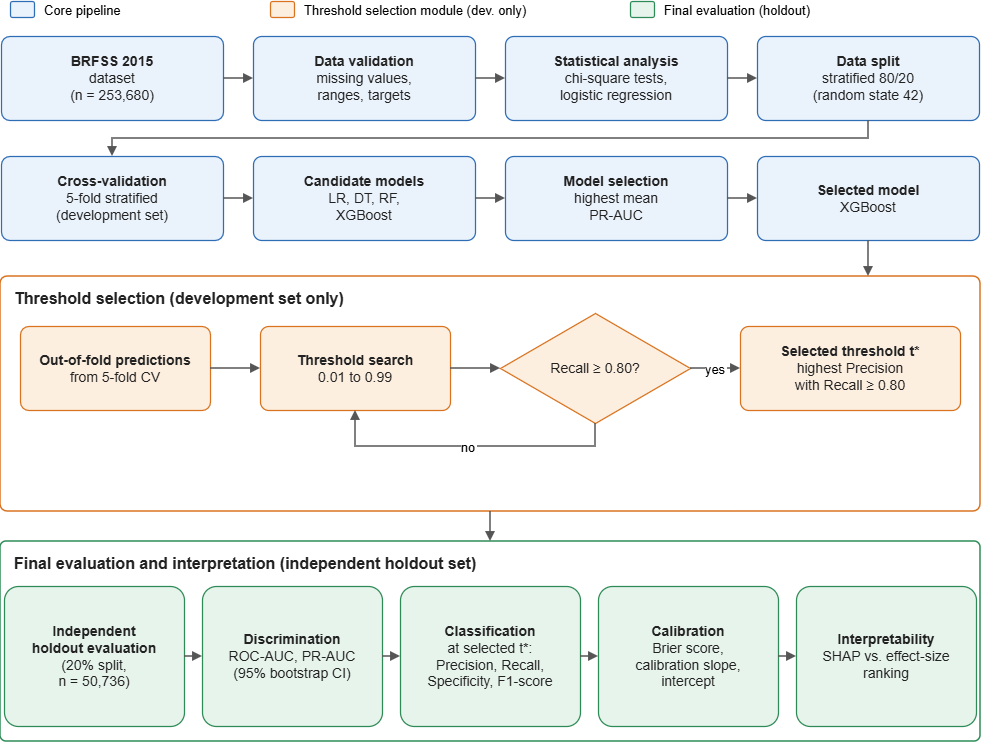
\includegraphics[
    width=\linewidth,
    keepaspectratio
]{images/pipeline_method.png}
\caption{Analysis workflow used for statistical inference, model selection,
holdout evaluation, calibration assessment, and model explanation.}
\label{fig:methodology_pipeline}
\end{figure}


\subsection{Dataset and Data Validation}
\label{subsec:dataset}


The CDC BRFSS 2015 Diabetes Health Indicators dataset contained
\textbf{253,680 records} and 21 predictors~\citep{cdc2015brfss,uci2023cdc,teboul2021kaggle}.
The original data sources are documented in the project repository.
The binary target combined reported prediabetes and diabetes into Class 1,
while Class 0 represented no reported diabetes.
Class 1 contained \textbf{35,346 records (13.93\%)}, and Class 0 contained
218,334 records (86.07\%).

Validation checks covered missing values, data types, target values, and
feature ranges.
No missing or out-of-range values were identified.
Variables stored as floating-point values despite having integer-valued
entries were converted to integer format.

The data integrity audit identified \textbf{24,206 surplus exact duplicate
rows} across all 22 columns, including the target variable.
When considering only the 21 predictors, \textbf{25,772 surplus observations}
were identified among repeated predictor profiles.
These counts represent different definitions of duplication and are not
mutually exclusive.
All records were retained because respondent identifiers were unavailable,
and identical survey responses could not be reliably attributed to the
same individual.
Removing these observations could therefore exclude valid responses
from distinct respondents.

No SMOTE, oversampling, or undersampling was applied.
All analyses therefore used the observed class distribution.


\subsection{Statistical Association Analysis}
\label{subsec:stats}

Univariate tests were selected according to variable type.
Eighteen binary, categorical, or ordinal predictors were evaluated using
the Chi-Square Test of Independence.
Association strength was measured with Cram{\'e}r's $V$:

\begin{equation}
V =
\sqrt{
\frac{\chi^2}
{N \cdot \min(r-1,c-1)}
}.
\end{equation}

For interpretation, $V<0.05$ was treated as negligible,
0.05--$<0.10$ as weak,
0.10--$<0.20$ as small,
0.20--$<0.30$ as moderate,
and $\geq0.30$ as strong.

BMI, mental unhealthy days, and physical unhealthy days were treated as
numerical variables.
Group differences were evaluated using Welch's two-sample $t$-test and the
Mann--Whitney U test.
Cohen's $d$, rank-biserial correlation, and common-language effect size
were used to describe effect magnitude.
Absolute rank-biserial correlation was used when ranking numerical
predictors by univariate effect size.

Holm correction was applied jointly across the 18 Chi-Square tests
and three Mann--Whitney U tests.
Effect sizes were interpreted alongside adjusted $p$-values because the
large sample size could produce small $p$-values for weak associations.

A multivariable Logistic Regression model containing all 21 predictors was
also fitted to estimate adjusted associations.
Reported quantities included regression coefficients, adjusted odds
ratios, 95\% confidence intervals, Holm-adjusted $p$-values, and variance
inflation factors.
For binary predictors, an odds ratio compared values 1 and 0.
For numerical predictors, it represented a one-unit increase.
For categorical predictors represented by dummy variables, each odds
ratio compared a category with its reference category.
These estimates were treated as sample-level associations and not as
causal effects.


\subsection{Model Development and Selection}
\label{subsec:ml}

The dataset was divided using a stratified 80/20 split with random state
42.
The development set contained \textbf{202,944 records}, and the independent
internal holdout set contained \textbf{50,736 records}.
The holdout set was excluded from model selection, feature selection,
threshold selection, and model-fitting decisions.

Four classifiers were compared using scikit-learn and XGBoost implementations~\citep{pedregosa2011scikit,chen2016xgboost}:
Logistic Regression, Decision Tree, Random Forest, and XGBoost.
Five-fold stratified cross-validation was performed only on the development
set.

For predictive Logistic Regression, BMI, mental unhealthy days, and
physical unhealthy days were standardized.
GenHlth, Age, Education, and Income were one-hot encoded, while binary
variables were retained without scaling.
Tree-based models used the original encoded feature values.

The prespecified model configurations were:
Logistic Regression with a maximum of 1,000 iterations;
Decision Tree with maximum depth 8;
Random Forest with 100 trees and maximum depth 12; and
XGBoost with 100 boosting rounds, maximum depth 6, and learning rate 0.1.

Accuracy, Precision, Recall, F1-score, ROC-AUC, and PR-AUC were calculated
for each fold.
\textbf{Mean PR-AUC, computed as average precision, was the primary
model-selection metric} because Class 1 represented 13.93\% of the dataset.
Mean ROC-AUC and lower PR-AUC variability were prespecified as tie-breakers.


\subsection{Threshold Selection and Holdout Evaluation}
\label{subsec:threshold}

After model selection, out-of-fold probabilities were generated for every
record in the development set.
Candidate thresholds from 0.01 to 0.99 were evaluated without using the
holdout set.

Thresholds satisfying
\[
\mathrm{Recall} \geq 0.80
\]
were retained.
Among these candidates, the threshold with the highest Precision was
selected.
F1-score and then the higher threshold were used as tie-breakers.

After the model and threshold were fixed, the selected classifier was
trained on the complete development set and evaluated once on the
independent holdout set.
Reported metrics included Accuracy, Precision, Recall, Specificity,
F1-score, ROC-AUC, PR-AUC, and the confusion matrix.

Uncertainty was estimated with
\textbf{1,000 stratified bootstrap samples} drawn from the holdout set.
Percentile-based 95\% confidence intervals were calculated for ROC-AUC,
PR-AUC, Recall, Precision, and F1-score.



\subsection{Calibration and SHAP Analysis}
\label{subsec:calibration_shap}

Calibration was evaluated on the holdout set using the Brier score, calibration slope, intercept, and a reliability curve with 10 probability groups. The slope and intercept were estimated by regressing observed outcomes on the log-odds of predicted probabilities. No probability recalibration was applied.

SHAP values were calculated using TreeExplainer for the final XGBoost model. The original stratified split was reconstructed, and up to 10,000 holdout records were sampled with random state 42. Global feature importance was measured by the mean absolute SHAP value.

SHAP importance was compared primarily with likelihood-ratio Chi-square statistics from multivariable Logistic Regression. For each predictor, the statistic measured the change in model fit after removing that predictor, including its entire dummy-variable block for categorical features:

\begin{equation}
\Delta D_j =
2\left(
\ell_{\mathrm{full}} -
\ell_{\mathrm{reduced},j}
\right),
\end{equation}

where $\ell_{\mathrm{full}}$ and $\ell_{\mathrm{reduced},j}$ represent the log-likelihoods of the full and reduced models. These values were used to rank the adjusted contributions of all 21 predictors.

Ranking agreement was assessed through Top-5, Top-10, and Top-15 overlap, Jaccard similarity, and Spearman rank correlation. To account for differences in predictor degrees of freedom, additional comparisons used $\chi^2-\mathrm{df}$ and $\chi^2/\mathrm{df}$.

A supplementary comparison used univariate effect sizes: Cram{\'e}r's $V$ for categorical and ordinal predictors, and absolute rank-biserial correlation for numerical predictors. Marginal associations were considered non-negligible at $V\geq0.05$ or $|r_{\mathrm{rb}}|\geq0.10$.

These comparisons examined agreement between statistical and model-based importance measures, not clinical validity or causality.




\section{Results}\label{sec:results}

\subsection{Statistical Association Results}
\label{subsec:stat_results}

Among the categorical and ordinal variables, the largest associations with
the target were observed for \textbf{\textit{GenHlth} ($V=0.2993$)},
\textbf{\textit{HighBP} ($V=0.2631$)},
\textit{DiffWalk} ($V=0.2183$), and
\textit{HighChol} ($V=0.2003$).
Age showed a smaller association ($V=0.1862$).
Several other variables remained statistically significant after Holm
correction but had weak or negligible effect sizes.

\begin{figure}[htbp]
\centering
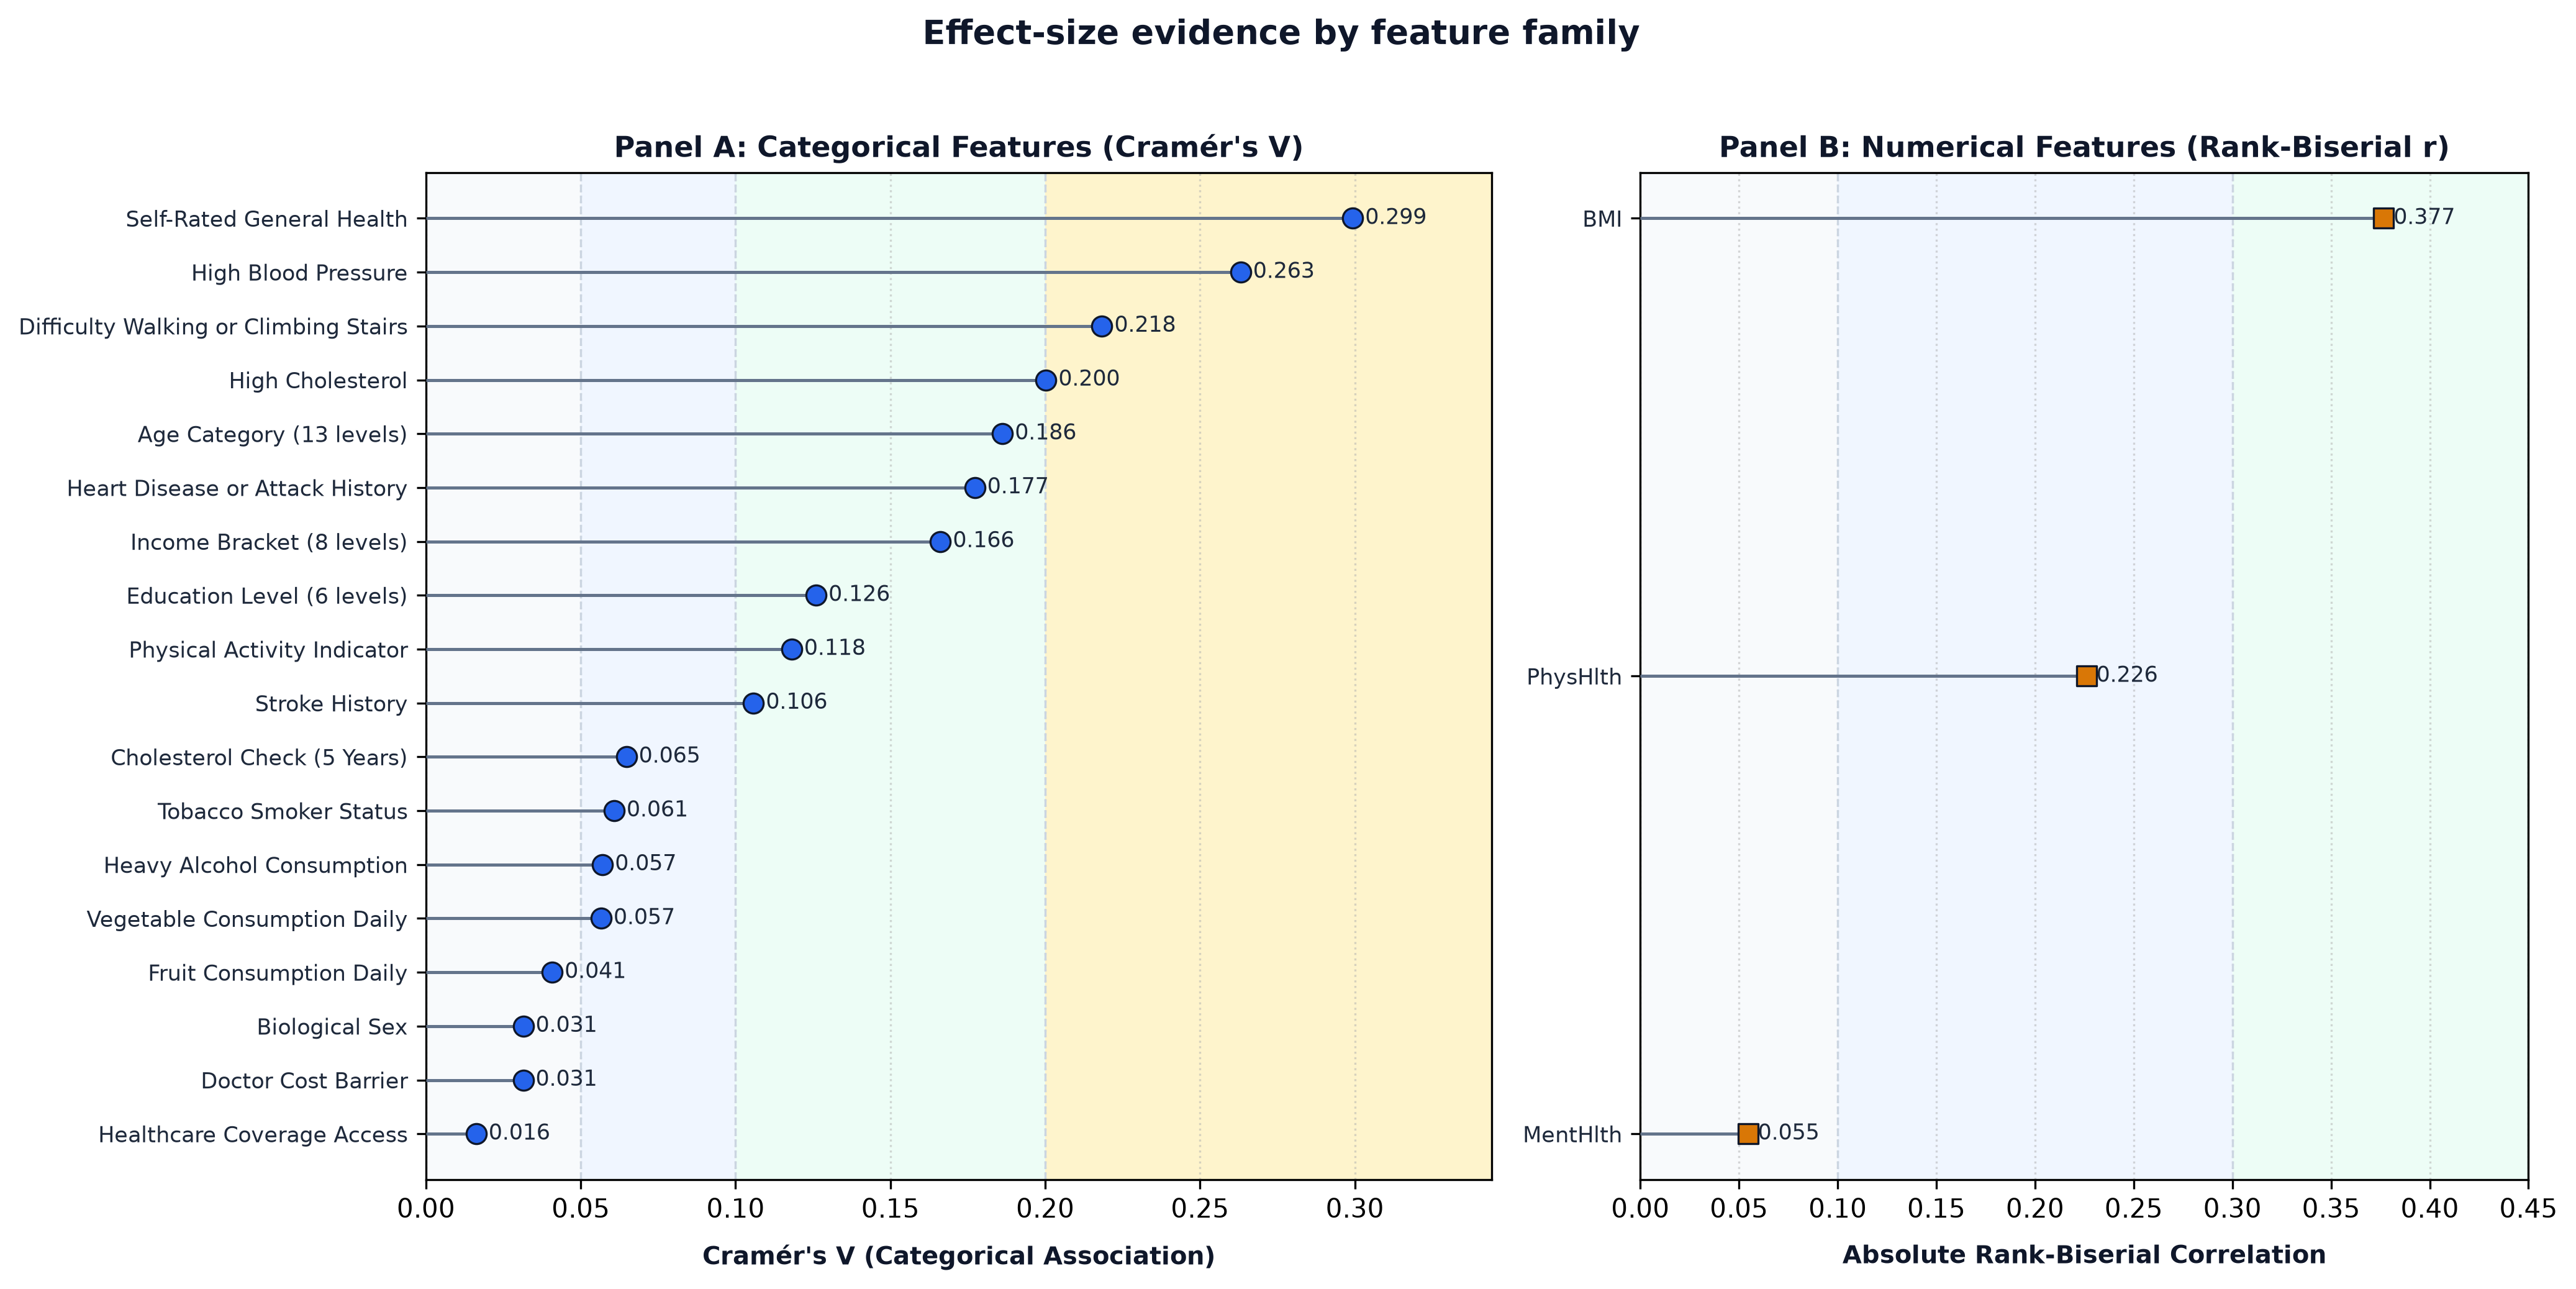
\includegraphics[
    width=\linewidth,
    keepaspectratio
]{images/effect_size_ranking.png}
\caption{Univariate effect-size rankings by feature family. Categorical and ordinal predictors are ranked by Cram{\'e}r's $V$, while numerical predictors are ranked by absolute rank-biserial correlation. Larger values indicate stronger marginal association within the analyzed sample.}
\label{fig:cramers_v_ranking}
\end{figure}

For the numerical variables, BMI showed the largest difference between the
two classes, followed by physical unhealthy days.
Mental unhealthy days had a smaller distributional effect
(Table~\ref{tab:numerical}).

\begin{table}[htbp]
\centering
\caption{Numerical Feature Comparisons Between Target Classes}
\label{tab:numerical}
\footnotesize
\renewcommand{\arraystretch}{1.4}
\setlength{\tabcolsep}{5pt}

\begin{tabularx}{\linewidth}{lYYYYY}
\toprule
Variable &
Class 0 &
Class 1 &
Cohen's $d$ &
Rank-biserial $r$ &
CLES \\
\midrule

\textbf{BMI} &
27.81 &
\textbf{31.94} &
\textbf{0.6414} &
\textbf{0.3766} &
\textbf{0.6883} \\

PhysHlth &
3.64 &
7.95 &
0.5022 &
0.2260 &
0.6130 \\

MentHlth &
2.98 &
4.46 &
0.2006 &
0.0546 &
0.5273 \\

\bottomrule
\end{tabularx}

\vspace{1mm}

\begin{minipage}{\linewidth}
\scriptsize
\textit{Note.}
Class 0 denotes no reported diabetes; Class 1 denotes reported prediabetes
or diabetes. All three Mann--Whitney U comparisons remained significant
after Holm correction.
\end{minipage}
\end{table}

The multivariable Logistic Regression included all 21 predictors.
Seventeen predictors had significant feature-level likelihood-ratio tests
after Holm correction. The maximum VIF reached \textbf{357.58}
for the \textit{Education\_6} dummy variable.
The largest positive adjusted odds ratios among the reported binary predictors
were observed for
\textbf{\textit{CholCheck}, OR = 3.4378}
(95\% CI: 3.0055--3.9321),
\textbf{\textit{HighBP}, OR = 2.0482}
(95\% CI: 1.9898--2.1083),
and \textit{HighChol}, OR = 1.7094.
For \textit{GenHlth}, category 5 had an OR of 7.5900
(95\% CI: 6.9851--8.2471) relative to category 1.

For binary predictors, odds ratios compare values 1 and 0.
For categorical dummy variables, they compare a category with the
reference category. High VIFs for some dummy variables require caution
when interpreting individual regression coefficients.
These estimates describe adjusted associations within the analyzed sample
and do not establish causal effects.


\subsection{Cross-Validated Model Selection}
\label{subsec:ml_results}

The four classifiers were compared using five-fold stratified
cross-validation on the development set, with mean PR-AUC as the primary
selection metric.

XGBoost achieved the highest mean
\textbf{PR-AUC of 0.4359} and
\textbf{ROC-AUC of 0.8305}.
Random Forest had the second-highest PR-AUC at 0.4301, a difference of
0.0058 from XGBoost.

\begin{table}[htbp]
\centering
\caption{Five-Fold Cross-Validation Performance on the Development Set}
\label{tab:model_comparison}
\footnotesize
\renewcommand{\arraystretch}{1.4}
\setlength{\tabcolsep}{7pt}

\begin{tabularx}{\linewidth}{lYY}
\toprule
Model & PR-AUC (mean $\pm$ SD) & ROC-AUC (mean $\pm$ SD) \\
\midrule

Logistic Regression & 0.4163 $\pm$ 0.0052 & 0.8250 $\pm$ 0.0016 \\
Decision Tree       & 0.4015 $\pm$ 0.0065 & 0.8169 $\pm$ 0.0025 \\
Random Forest       & 0.4301 $\pm$ 0.0070 & 0.8271 $\pm$ 0.0024 \\
\textbf{XGBoost}    & \textbf{0.4359 $\pm$ 0.0077} & \textbf{0.8305 $\pm$ 0.0021} \\

\bottomrule
\end{tabularx}

\vspace{1mm}

\begin{minipage}{\linewidth}
\scriptsize
\textit{Note.}
Values are mean $\pm$ standard deviation across five stratified folds.
PR-AUC was the prespecified primary model-selection metric; mean ROC-AUC and then lower PR-AUC variability were used only as tie-breakers.
\end{minipage}
\end{table}

\begin{figure}[htbp]
\centering
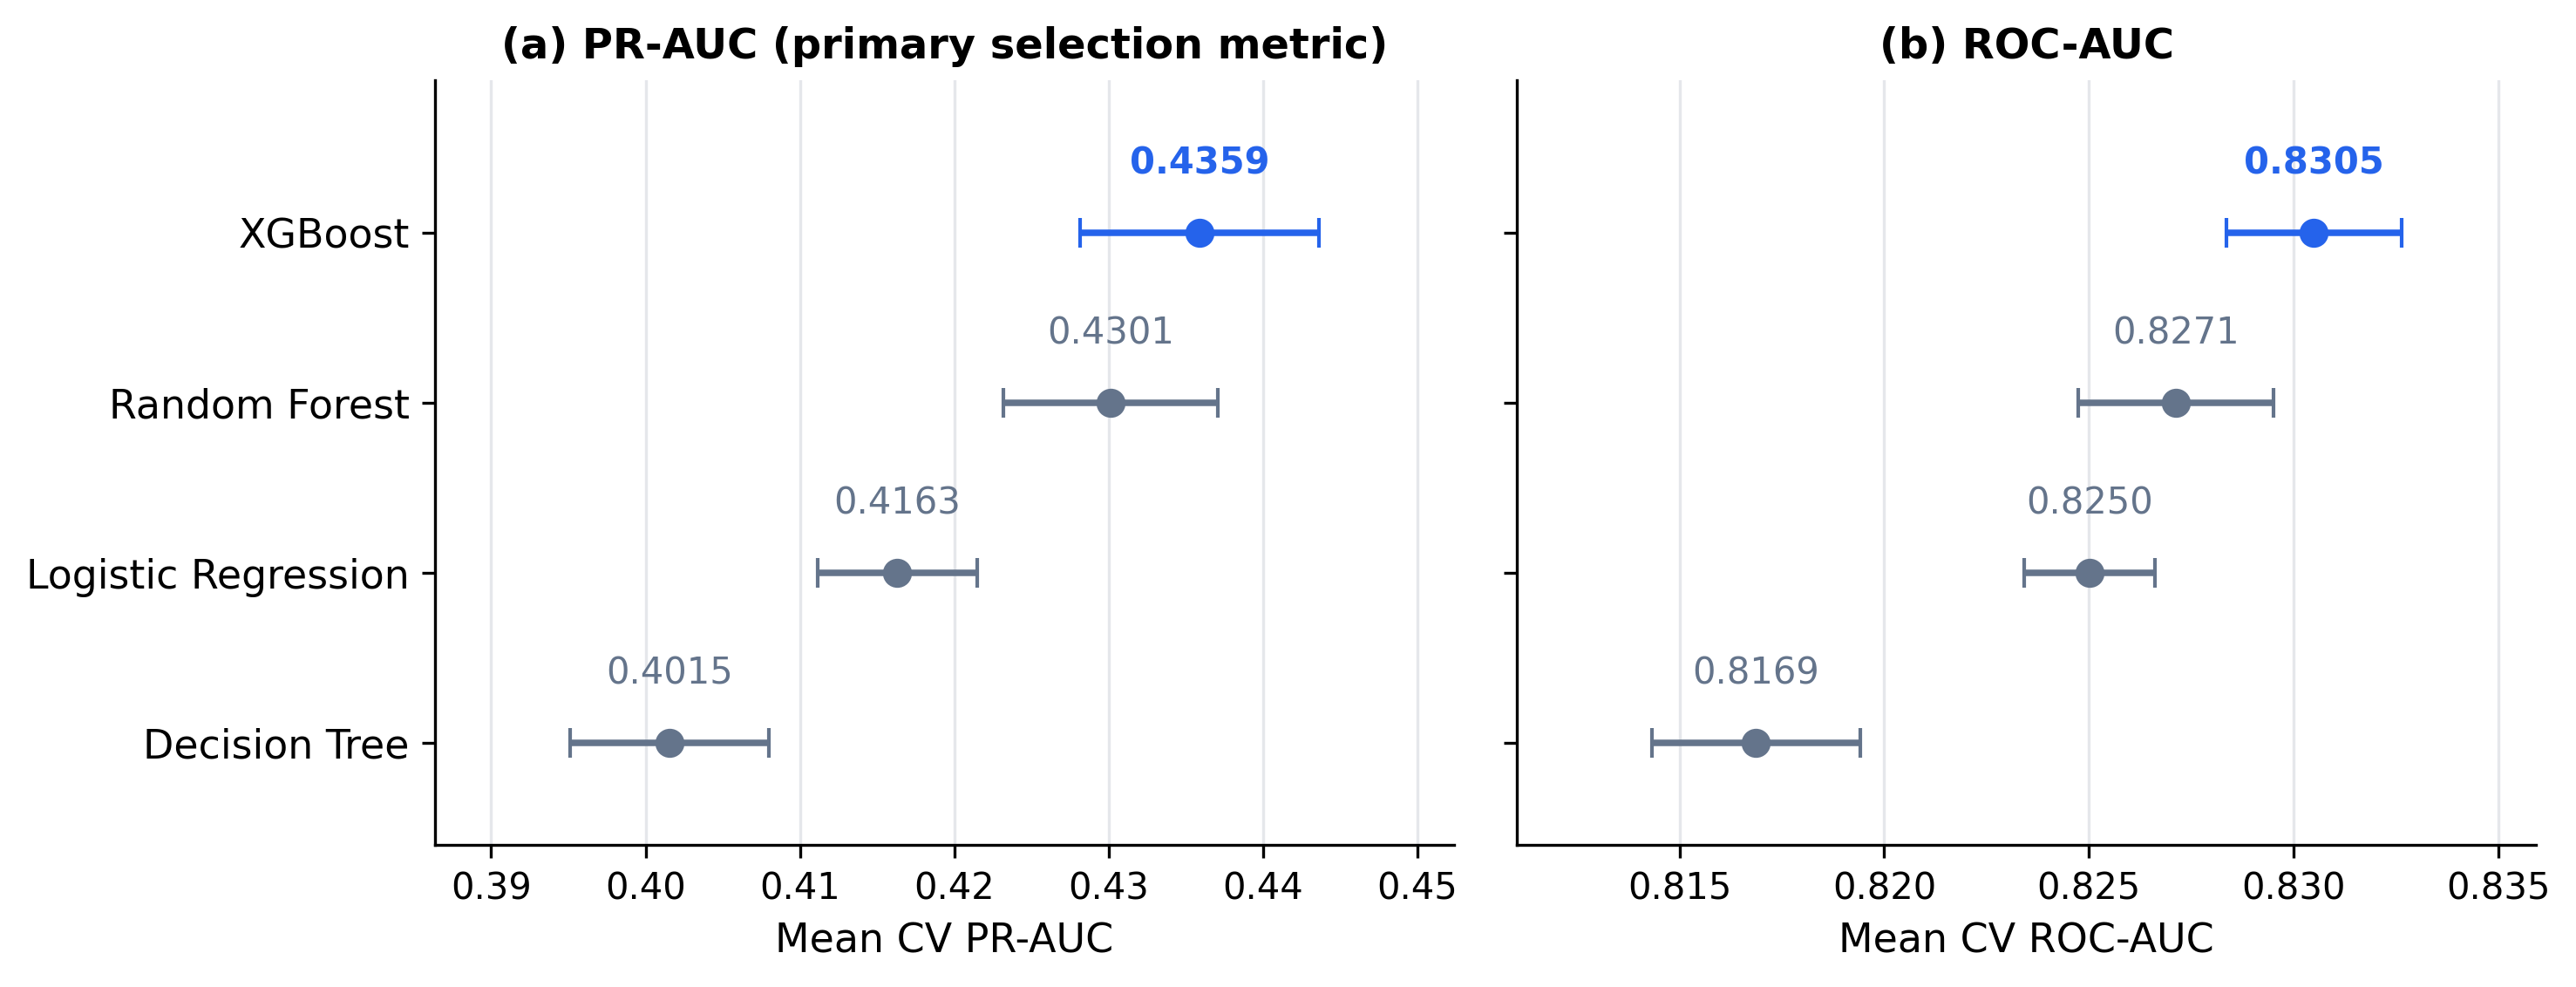
\includegraphics[
    width=\linewidth,
    keepaspectratio
]{images/cv_model_comparison.png}
\caption{Cross-validated PR-AUC and ROC-AUC for the four classifiers.}
\label{fig:cv_model_comparison}
\end{figure}

XGBoost was therefore selected for threshold analysis and final holdout
evaluation.


\subsection{Threshold Selection, Holdout Performance, and Calibration}
\label{subsec:holdout_results}

The classification threshold was selected from out-of-fold development
predictions before the holdout set was evaluated.
Among thresholds satisfying Recall $\geq 0.80$, the highest Precision was
obtained at \textbf{0.13}.

On the independent internal holdout set, lowering the threshold from 0.50
to 0.13 increased Recall from 0.1654 to
\textbf{0.8099}, while Precision decreased from 0.5583 to
\textbf{0.2991}.
False negatives decreased from 5,900 to
\textbf{1,344}, whereas false positives increased from 925 to
\textbf{13,416}.

\begin{table}[htbp]
\centering
\caption{Holdout Performance at the Default and Selected Thresholds}
\label{tab:threshold_comparison}
\footnotesize
\renewcommand{\arraystretch}{1.4}
\setlength{\tabcolsep}{8pt}

\begin{tabularx}{\linewidth}{lYY}
\toprule
Metric & Threshold 0.50 & \textbf{Threshold 0.13} \\
\midrule

Accuracy      & 0.8655 & 0.7091 \\
Precision     & 0.5583 & 0.2991 \\
Recall        & 0.1654 & \textbf{0.8099} \\
Specificity   & 0.9788 & 0.6928 \\
F1-score      & 0.2552 & \textbf{0.4369} \\
True positives & 1,169 & 5,725 \\
True negatives & 42,742 & 30,251 \\
False negatives & 5,900 & \textbf{1,344} \\
False positives & 925 & 13,416 \\

\bottomrule
\end{tabularx}
\end{table}

The threshold-independent holdout metrics were
\textbf{ROC-AUC = 0.8272} and
\textbf{PR-AUC = 0.4238}.
Their 95\% bootstrap confidence intervals were
0.8223--0.8322 and 0.4135--0.4347, respectively.
At threshold 0.13, the bootstrap intervals were
0.8004--0.8194 for Recall,
0.2953--0.3028 for Precision, and
0.4317--0.4418 for F1-score.

\begin{figure}[htbp]
\centering
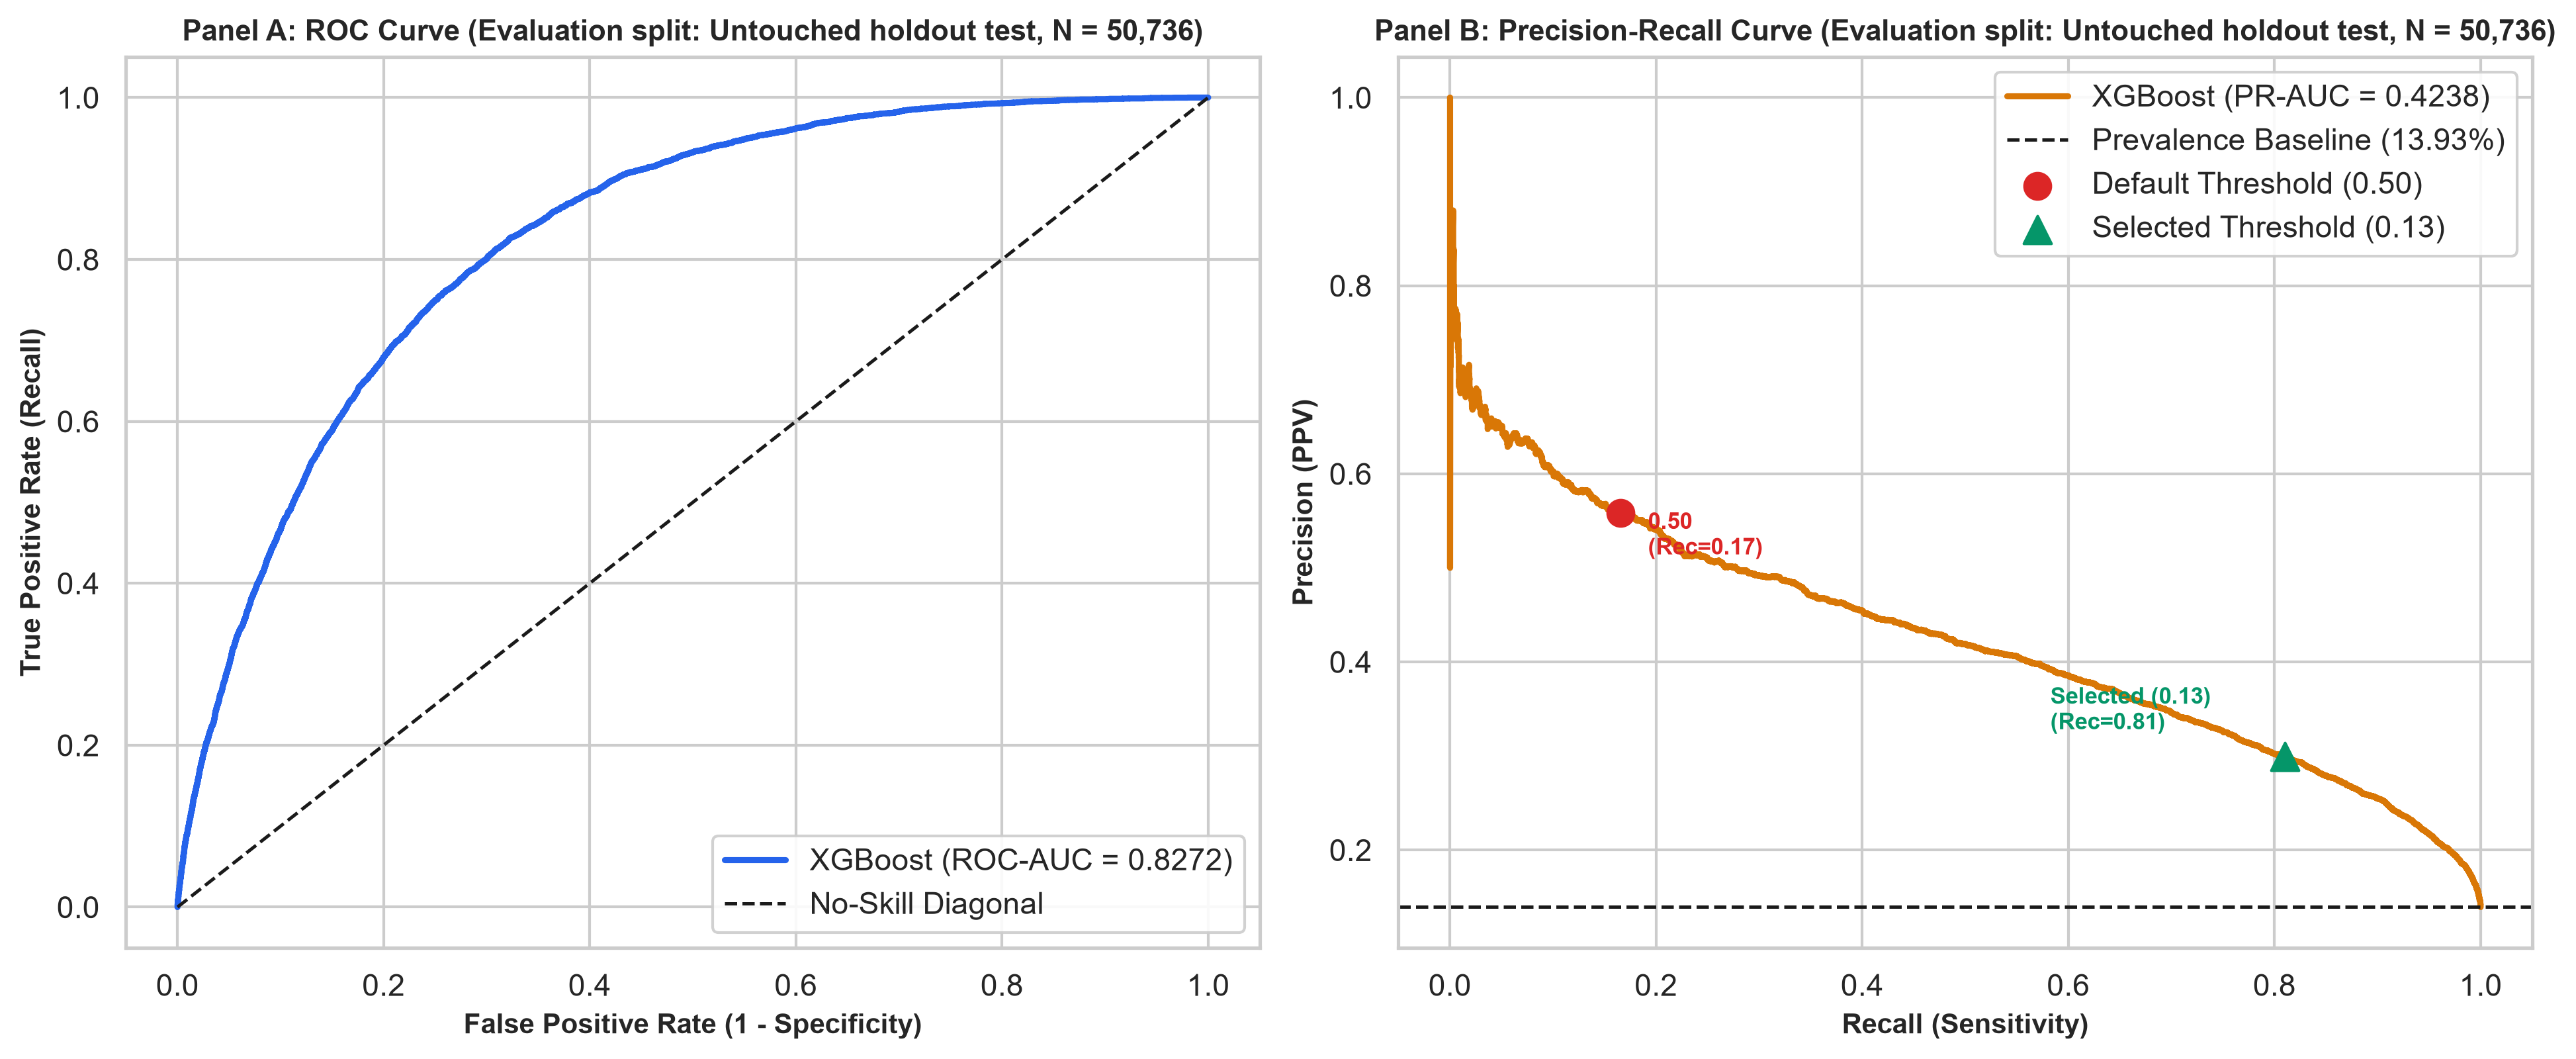
\includegraphics[
    width=\linewidth,
    keepaspectratio
]{images/holdout_roc_pr_curves.png}
\caption{ROC and Precision--Recall curves for XGBoost on the independent
internal holdout set.}
\label{fig:holdout_roc_pr}
\end{figure}

Calibration on the holdout set yielded a
\textbf{Brier score of 0.0974},
a \textbf{calibration slope of 0.9589}, and an
\textbf{intercept of $-0.0515$}.
No recalibration procedure was applied.


\subsection{SHAP Explanation and Evidence Alignment}
\label{subsec:shap_results}

The five highest-ranked features by mean absolute SHAP value were
\textbf{\textit{GenHlth}},
\textbf{\textit{HighBP}},
\textbf{Age},
\textbf{BMI}, and
\textbf{\textit{HighChol}}.
Their mean absolute SHAP values were 0.6381, 0.5264, 0.3994, 0.3978,
and 0.2927, respectively.

Higher encoded \textit{GenHlth} scores, high blood pressure, older age,
and higher BMI more often produced positive SHAP contributions.
These values describe contributions to the fitted model prediction and do
not estimate causal effects.

\begin{figure}[htbp]
\centering
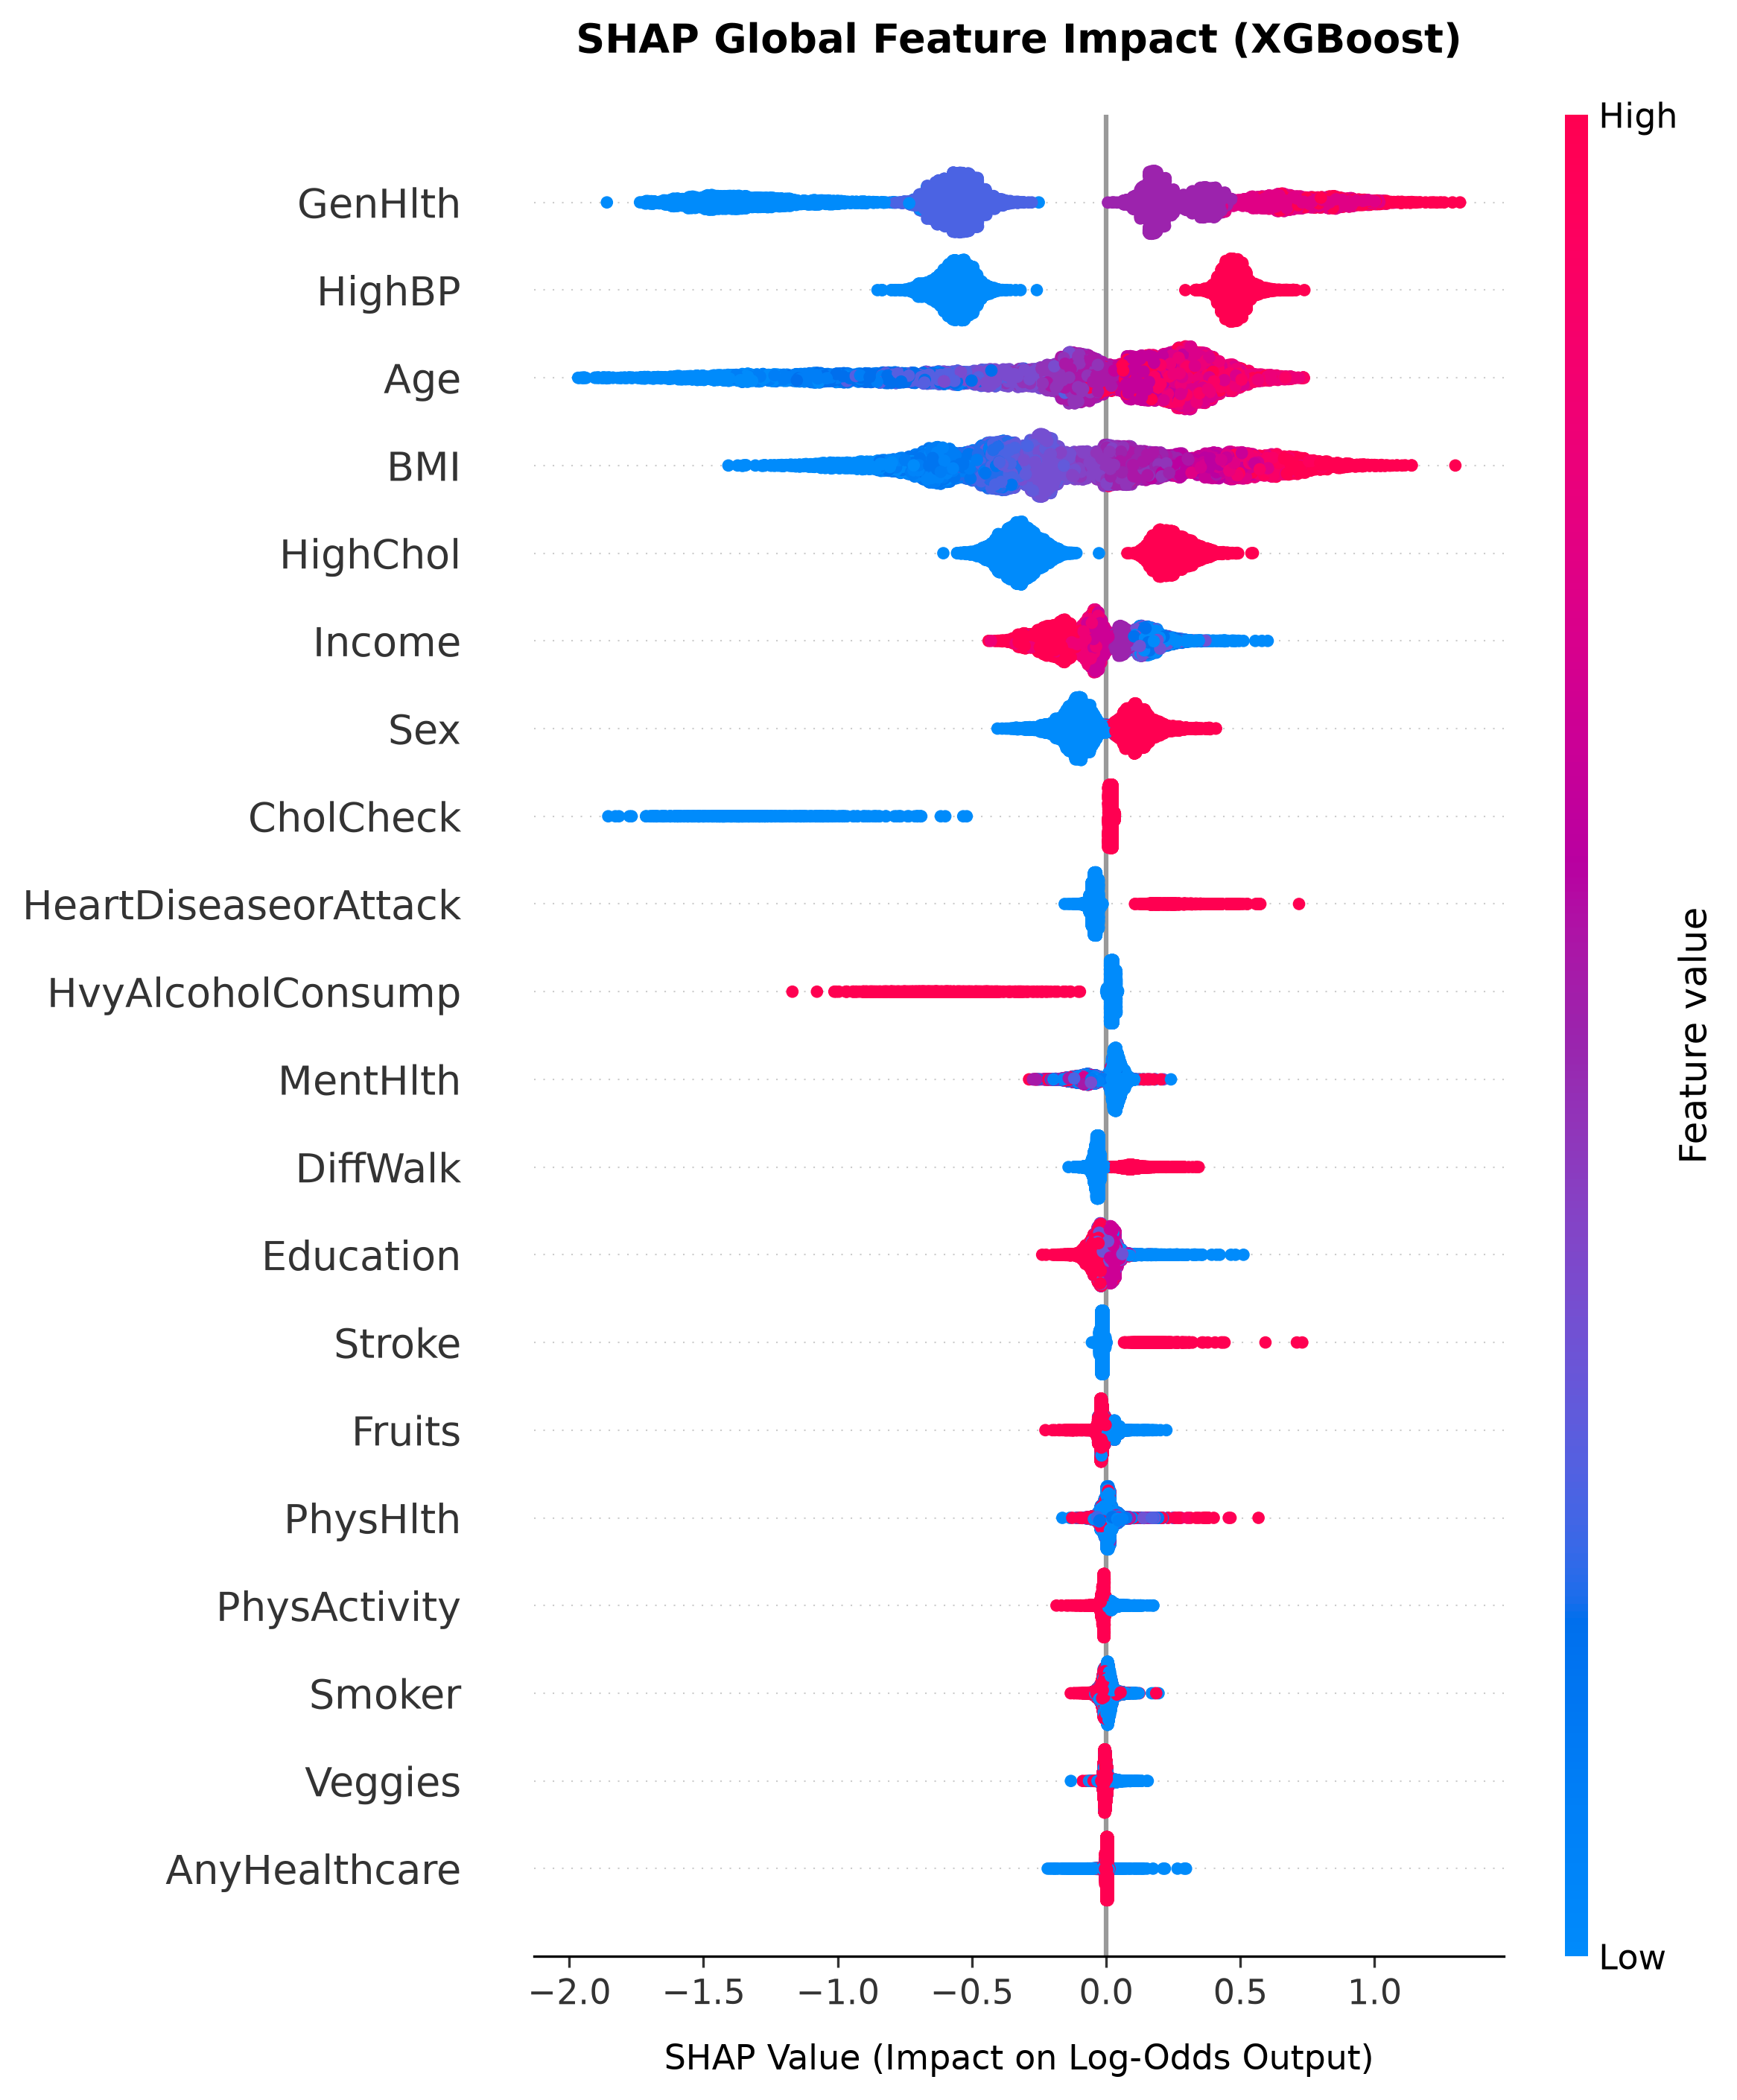
\includegraphics[
    width=0.45\linewidth,
    keepaspectratio
]{images/shap_summary_beeswarm.png}
\caption{SHAP summary plot for the final XGBoost model.}
\label{fig:shap_beeswarm}
\end{figure}


The primary evidence-alignment analysis compared global SHAP
importance with feature-level likelihood-ratio Chi-square
contributions from multivariable Logistic Regression.
The Top-5 and Top-10 rankings contained identical feature sets,
yielding overlaps of 5/5 and 10/10, respectively.
The Top-10 Jaccard similarity was \textbf{1.0000}.

Across all 21 predictors, the two rankings showed a
\textbf{Spearman rank correlation of $r_s=0.9338$}
($p=6.38\times10^{-10}$).
The Top-15 rankings shared 13 features, with a Jaccard
similarity of 0.7647.

The ten shared Top-10 features were \textit{GenHlth},
\textit{HighBP}, Age, BMI, \textit{HighChol}, Income,
Sex, \textit{CholCheck}, \textit{HeartDiseaseorAttack},
and \textit{HvyAlcoholConsump}.

Sensitivity analysis accounting for predictor degrees of freedom
showed that the $\chi^2-\mathrm{df}$ ranking retained complete
Top-10 overlap with SHAP.
Using $\chi^2/\mathrm{df}$ reduced the overlap to 9/10
(Jaccard similarity = 0.8182), while Spearman rank correlation
remained 0.8818.

\begin{figure}[htbp]
\centering
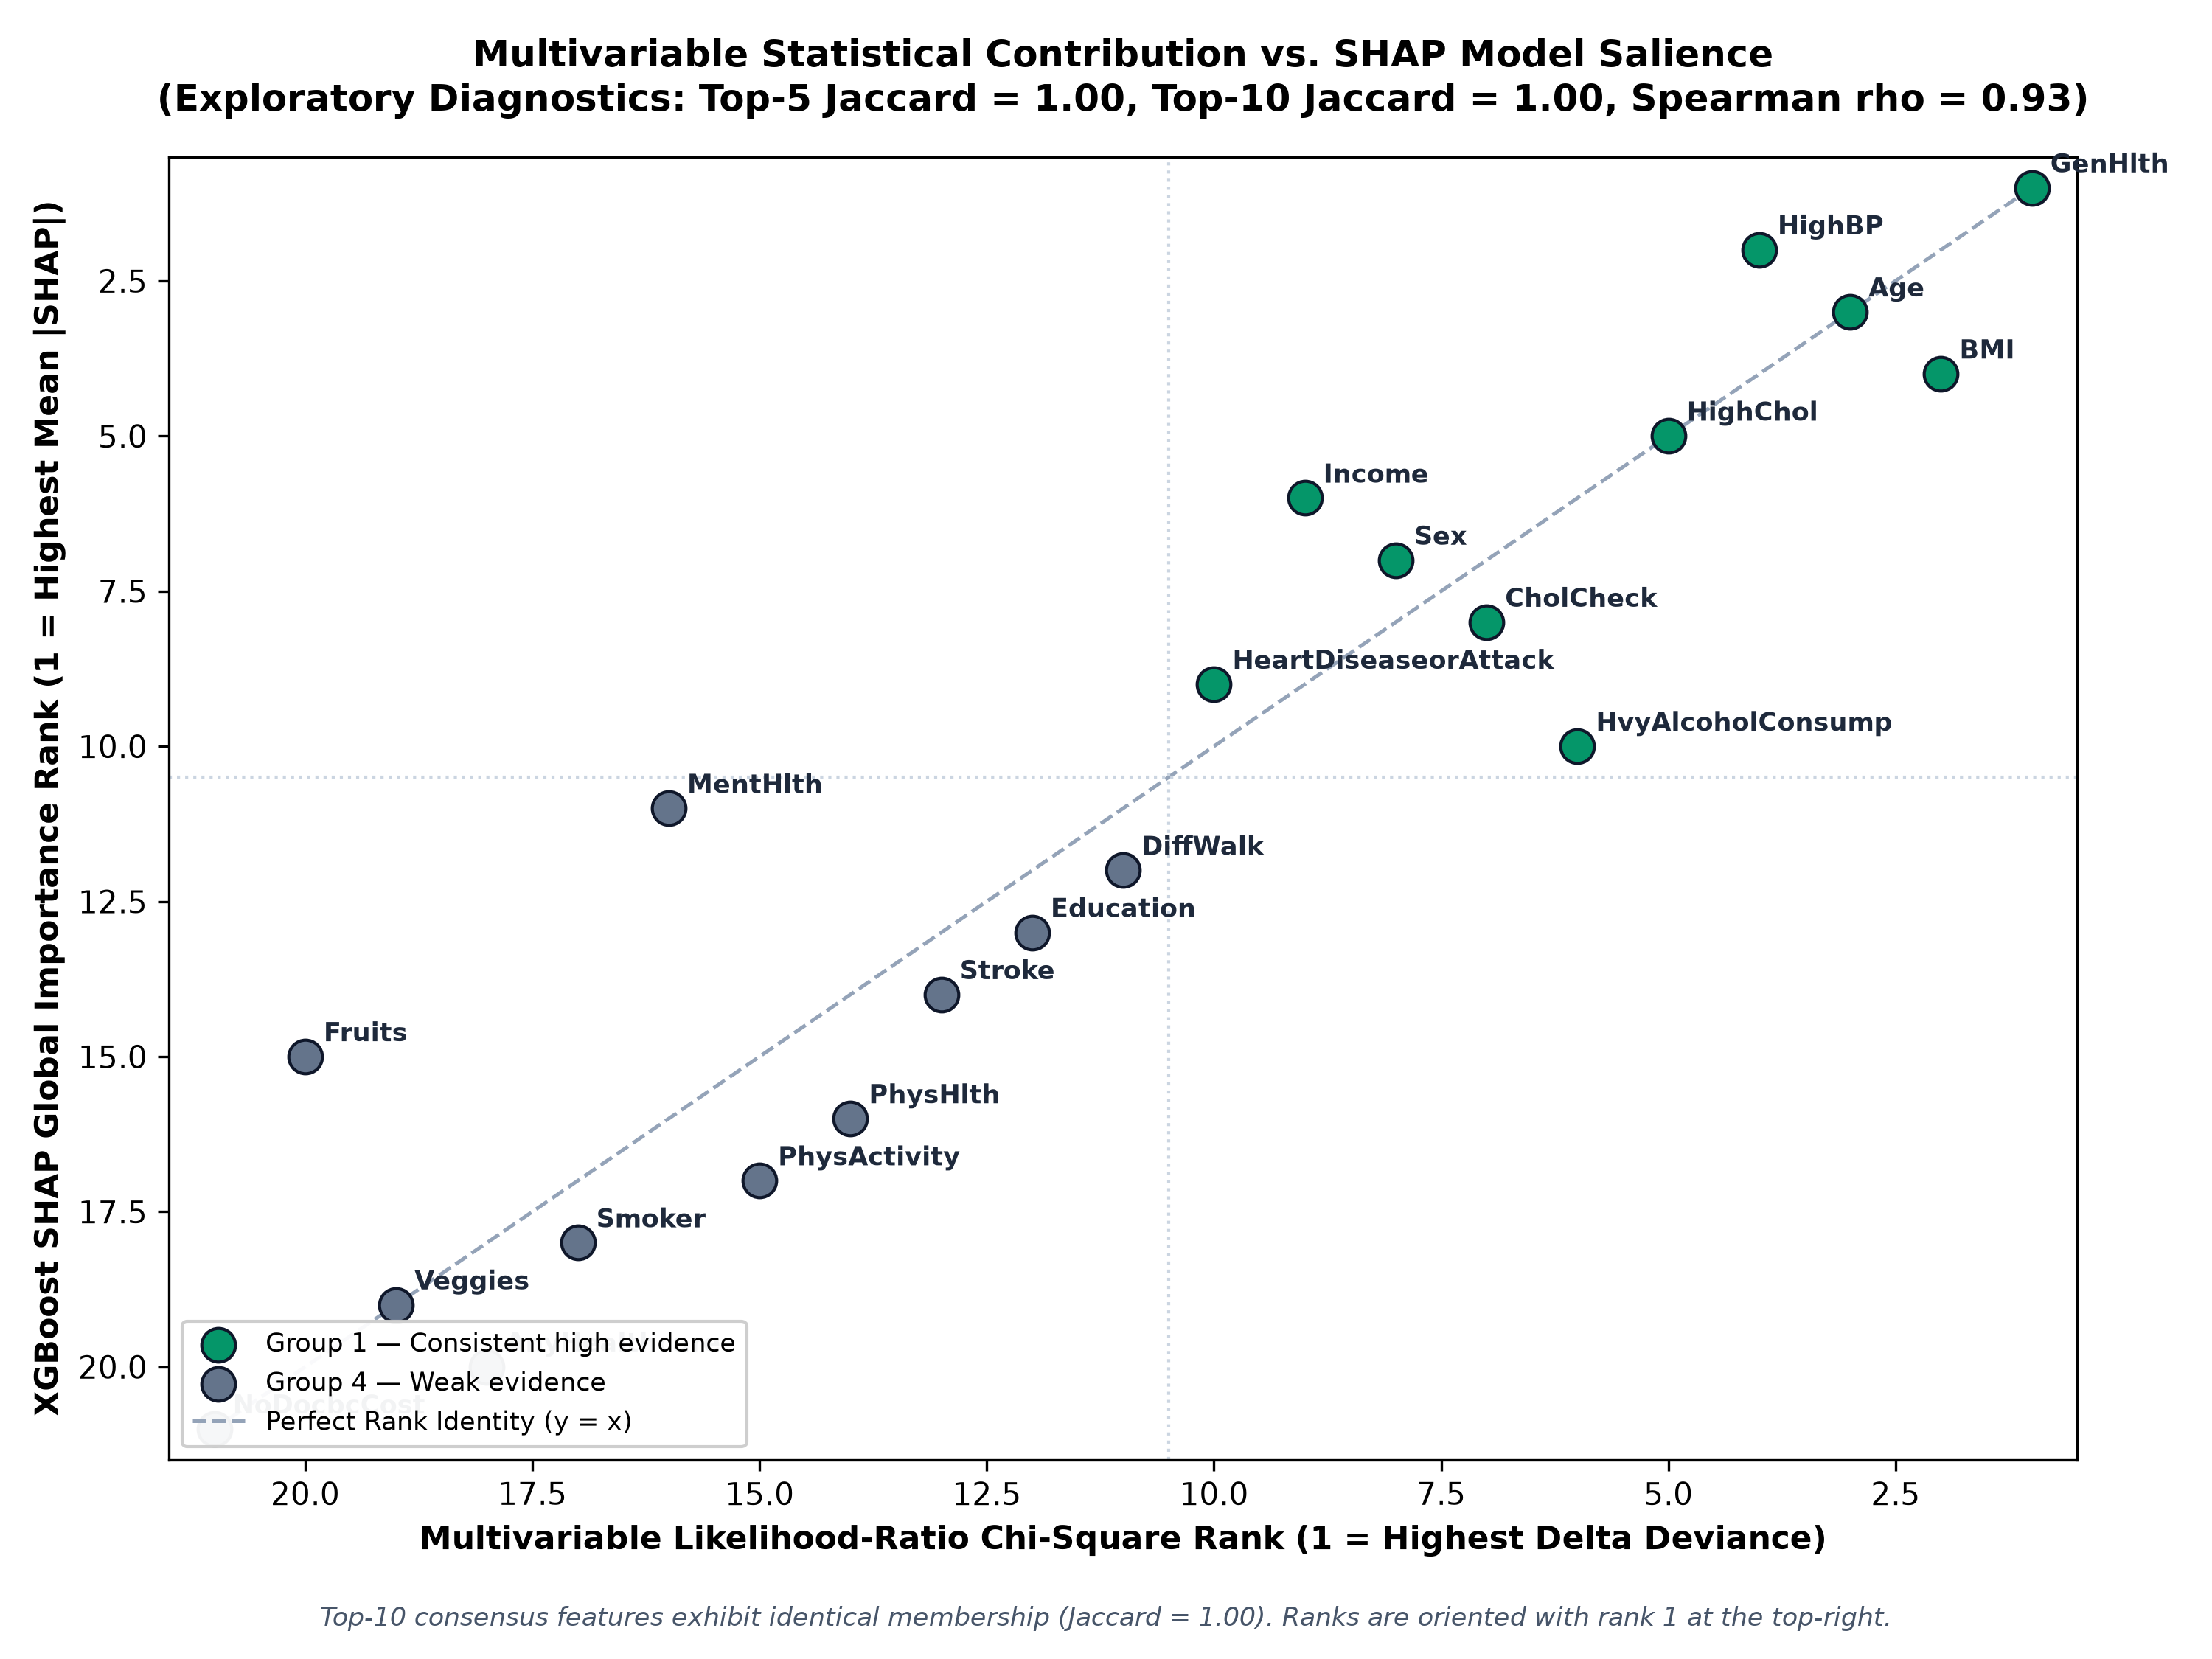
\includegraphics[
    width=0.7\linewidth,
    keepaspectratio
]{effect_size_shap_alignment.png}
\caption{Exploratory alignment between global SHAP importance
and feature-level multivariable likelihood-ratio Chi-square
contributions. Rankings are based on 21 predictors, with
lower rank values indicating greater importance.
The comparison describes internal rank agreement rather than
independent clinical validation.}
\label{fig:evidence_alignment}
\end{figure}

The supplementary comparison with univariate effect sizes
showed lower agreement.
The Top-5, Top-10, and Top-15 rankings shared 3, 7, and
12 features, respectively.
The Top-10 overlap corresponded to a
\textbf{Jaccard similarity of 0.5385}.
Nine of the ten highest-ranked SHAP features met the
prespecified threshold for non-negligible marginal association.

Differences between the univariate and SHAP rankings were
observed for several predictors.
For example, \textit{DiffWalk} had Cram{\'e}r's $V=0.2183$
but ranked 12th by SHAP, whereas Sex ranked seventh by SHAP
despite a marginal Cram{\'e}r's $V=0.0314$.

These results show that SHAP importance was more closely
aligned with adjusted multivariable likelihood-ratio
contributions than with univariate effect-size rankings
in the analyzed dataset.
The comparisons quantify different properties and do not
establish causal relationships or clinical relevance.


\section{Discussion}
\label{sec:discussion}

Three findings require interpretation.
First, XGBoost was selected under the prespecified cross-validation rule,
although its mean PR-AUC differed from Random Forest by only 0.0058.
Second, the development-selected threshold of 0.13 substantially changed
the balance between missed positive cases and false-positive predictions.

Third, global SHAP importance showed strong agreement with multivariable likelihood-ratio contributions, while the supplementary comparison with univariate effect sizes revealed less complete agreement.



\subsection{Model Selection, Screening Threshold, and Calibration}
\label{subsec:model_discussion}

XGBoost had the highest mean cross-validated PR-AUC, but the absolute
difference from Random Forest was small.
The selection should therefore be interpreted as the outcome of the
prespecified model-selection rule rather than evidence of a large
performance advantage over Random Forest.

The threshold analysis produced a larger practical change than the choice
between the two highest-ranked models.
At the default threshold of 0.50, the model detected only 16.54\% of the
positive holdout records.
Using the development-selected threshold of
\textbf{0.13 increased Recall to 80.99\%}, while
\textbf{Precision decreased to 29.91\%}.
False negatives decreased from 5,900 to 1,344, whereas false positives
increased from 925 to 13,416.

This threshold therefore represents a screening-oriented operating point
under the study's prespecified Recall constraint.
It should not be interpreted as a general clinical cutoff.
A setting in which false-positive follow-up is costly may require a
different threshold.

The threshold was selected exclusively from out-of-fold development
predictions before holdout evaluation.
This separation prevents direct optimization of the decision threshold on
the reported holdout results.

Calibration estimates on the internal holdout were
a Brier score of 0.0974, a slope of \textbf{0.9589}, and an intercept of
$-0.0515$.
The slope and intercept were close to their reference values of 1 and 0,
respectively, within this holdout sample.
These estimates do not establish calibration in another year, population,
or clinical setting.
No recalibration procedure was evaluated in the present analysis.




\subsection{Statistical Associations and SHAP Explanations}
\label{subsec:shap_discussion}

The statistical analysis and SHAP results pointed to the same five leading predictors: \textit{GenHlth}, \textit{HighBP}, Age, BMI, and \textit{HighChol}, although their order differed between XGBoost and multivariable Logistic Regression. All ten features in the Top-10 SHAP ranking also appeared in the likelihood-ratio Chi-square Top-10 (Jaccard similarity = 1.0000). Across all 21 predictors, Spearman rank correlation was $r_s=0.9338$.

Despite this close match, the methods measure different quantities. Likelihood-ratio statistics show how much the fit of Logistic Regression changes when a predictor is removed. SHAP describes each feature's contribution to XGBoost predictions. Matching feature sets does not mean that both methods assign the same meaning to feature importance. The ranking method also made a difference. Subtracting predictor degrees of freedom from likelihood-ratio statistics preserved the full Top-10 overlap, while dividing by degrees of freedom reduced it to nine features. The agreement was therefore strong, but partly depended on how statistical contribution was calculated.

The univariate effect-size comparison showed less agreement: only seven features appeared in both Top-10 rankings (Jaccard similarity = 0.5385). Unlike the multivariable analysis, these effect sizes describe each predictor separately. \textit{DiffWalk} and \textit{PhysHlth} had non-negligible marginal associations yet ranked 12th and 16th by SHAP. Sex showed the reverse pattern, ranking seventh by SHAP despite a small marginal association (Cram{\'e}r's $V=0.0314$).

Shared information among predictors or interactions captured by XGBoost may explain some differences. However, these mechanisms were not tested for individual features. The close agreement with multivariable likelihood-ratio rankings suggests that both fitted models placed high importance on a similar set of predictors in this dataset. It remains an internal comparison, not evidence that the SHAP explanations are clinically valid or that these predictors cause diabetes.




\subsection{Relation to Previous BRFSS Studies}
\label{subsec:literature_discussion}

\begin{table}[htbp]
\centering
\caption{Screening-oriented comparison with selected BRFSS studies.
Cross-study results are descriptive due to differences in
experimental settings.}
\label{tab:literature_comparison}

\footnotesize
\setlength{\tabcolsep}{5pt}
\renewcommand{\arraystretch}{1.4}

\begin{tabularx}{\linewidth}{
@{}p{3.6cm}
X
>{\centering\arraybackslash}p{1.5cm}
>{\centering\arraybackslash}p{1.5cm}@{}
}
\toprule
\textbf{Study} &
\textbf{Dataset / Model} &
\textbf{AUC (\%)} &
\textbf{Recall (\%)} \\
\midrule

\multicolumn{4}{@{}l}{
\textit{Previously published studies}
} \\

Xie et al.~\citep{xie2019diabetes} &
BRFSS 2014; Neural Network &
79.49 & 37.81 \\

Mohamed et al.~\citep{mohamed2024diabetes} &
BRFSS 2015; XGBoost &
82.00 & 19.00 \\

Li et al.~\citep{li2024gaxgboost} &
BRFSS-derived; Unbalanced XGBoost &
82.82 & 17.34 \\

Muhammad et al.~\citep{muhammad2025brfss} &
Tennessee 2023; Gradient Boosting &
80.00 & 32.00 \\

Majcherek et al.~\citep{majcherek2025aidriven} &
BRFSS 2015; Extra Trees / Resampling &
Up to 99 & 99.00 \\

\midrule

\multicolumn{4}{@{}l}{
\textbf{Present study: same independent holdout}
} \\

Present study &
XGBoost; Default ($t=0.50$) &
82.72 & 16.54 \\

\rowcolor{ourrow}
\textbf{Present study} &
\textbf{XGBoost; Selected ($t=0.13$)} &
\textbf{82.72} & \textbf{80.99} \\

\bottomrule
\end{tabularx}

\vspace{2mm}

\begin{minipage}{\linewidth}
\scriptsize
\textbf{Within-study screening improvement:}
Recall increased by \textbf{64.45 percentage points},
while missed positive cases decreased by
\textbf{77.22\%} (5,900 to 1,344).

\par\vspace{1mm}
\textit{Trade-off:}
Precision decreased from 55.83\% to 29.91\%.

\par\vspace{1mm}
\textit{Note.}
Published results use different datasets, class-balancing
strategies, and evaluation protocols and are not directly
rankable. Li et al.'s results shown here refer to the
unbalanced XGBoost setting; Majcherek et al.'s high
reported results involve different resampling and
evaluation configurations.
The threshold comparison for the present study uses
the same holdout predictions.
\end{minipage}

\end{table}


The proposed framework emphasizes screening sensitivity rather than maximizing overall accuracy. On the same independent holdout set, selecting the threshold from development-set out-of-fold predictions increased Recall from 16.54\% to \textbf{80.99\%}, reducing missed positive cases by \textbf{77.22\%}. This improvement came at the cost of lower Precision (29.91\%) and more false-positive predictions. Although several previous BRFSS studies reported higher classification performance under different experimental conditions, the main contribution of this work lies in its leakage-controlled threshold selection, explicit screening trade-off, and reliability-oriented evaluation rather than superiority in cross-study predictive accuracy.

The main contribution of the present study is consequently the evaluation
sequence rather than a new classifier: cross-validated model selection on the
development set, threshold selection from out-of-fold development predictions,
one-time internal holdout evaluation, bootstrap uncertainty, calibration
assessment, and an exploratory comparison of SHAP rankings with multivariable likelihood-ratio contributions, supplemented by univariate effect-size analysis. This framing is consistent with current guidance that
emphasizes transparent model evaluation and reporting rather than performance
claims based on a single metric~\citep{collins2024tripodai,moons2025probastai}.



\subsection{Limitations and Future Work}
\label{subsec:limitations}

The BRFSS 2015 dataset is cross-sectional and self-reported, without laboratory-confirmed diagnoses or survey weights. Consequently, the findings cannot establish causality or represent national population estimates. Future research should incorporate survey-weighted analyses and clinically validated data.

Model evaluation relied on an internal holdout from the same 2015 dataset. Although the development and holdout sets were separated, repeated predictor profiles could occur across partitions. Further validation using newer BRFSS waves or independent datasets is needed to assess generalizability.

The selected threshold of 0.13 reflects a specific Recall $\geq 0.80$ objective and should not be considered a universal clinical cutoff. Similarly, agreement between SHAP importance and statistical contributions does not establish clinical or causal validity. Future studies should evaluate decision thresholds under practical screening costs and examine explanation stability.




\section{Conclusion}\label{sec:conclusion}

The analysis used 253,680 records from the original imbalanced CDC BRFSS 2015 dataset. Repeated response profiles were retained because respondent identifiers were unavailable, preventing confirmation that matching records came from the same individuals. Among four models, XGBoost achieved the highest mean five-fold cross-validated PR-AUC (0.4359).

On the independent internal holdout set, XGBoost reached a PR-AUC of 0.4238 (95\% CI: 0.4135--0.4347) and ROC-AUC of 0.8272 (95\% CI: 0.8223--0.8322). A threshold of 0.13 was chosen using out-of-fold development predictions before holdout evaluation. Recall reached 80.99\% (95\% CI: 80.04\%--81.94\%), Precision 29.91\% (95\% CI: 29.53\%--30.28\%), Specificity 69.28\%, and F1-score 0.4369 (95\% CI: 0.4317--0.4418). Compared with the default threshold of 0.50, false negatives fell from 5,900 to 1,344, but false positives rose from 925 to 13,416. Calibration yielded a Brier score of 0.0974, slope of 0.9589, and intercept of $-0.0515$.

Multivariable Logistic Regression identified adjusted associations, though high VIFs for some categorical dummy variables call for caution when interpreting individual coefficients. SHAP ranked self-rated general health, high blood pressure, age, BMI, and high cholesterol highest in the fitted XGBoost model. SHAP and multivariable likelihood-ratio rankings shared all ten Top-10 features (Jaccard similarity = 1.0000; Spearman $r_s=0.9338$ across 21 predictors), compared with seven shared features for univariate effect sizes (Jaccard similarity = 0.5385).

The workflow brings together statistical analysis, development-only model and threshold selection, holdout evaluation, bootstrap uncertainty, calibration, and SHAP explanations. These results concern an unweighted BRFSS sample and do not establish clinical diagnosis, causality, or national population estimates. External validation with newer BRFSS waves, other populations, and datasets containing clinical biomarkers remains necessary.


\section*{Declaration}

Declaration of generative AI and AI-assisted technologies in the writing
process: generative AI tools were used for language editing only. The authors
reviewed and revised the manuscript and take full responsibility for the
accuracy and integrity of the work.

\backmatter

\bibliography{sn-bibliography}

\end{document}
